\section{Real-time estimation of vehicle state}
\label{sec:vehicle_model}

Real-time vehicle tracking has been the centre of much research, particularly for robotics applications and self-driving cars \citep{Daum_2005, Gustafsson_2002}. In many of these, data is sampled at a very high frequency, often multiple times per second, leading to highly accurate estimates of the object's \emph{state}.\footnote{State, as we discuss shortly, includes properties such as the \emph{speed} of the object.} Alas, with transit data this is seldom the case; instead, it is common for observations to be reported once every 10--30 seconds or, in some cases, even longer.

Low-frequency observations lead to high uncertainties of state parameters and difficulty capturing all possible trajectories, which can lead to degradation of the model and loss of information. In \cref{fig:vobs_multimode}, we show two possible trajectories for buses B and C; there are, in fact, countless possibilities: perhaps the bus waited at the stop a little longer? In this case, there is uncertainty about the bus's dwell time and speed; however, the first step of \agls{rbm} is to \emph{predict} the upcoming state \emph{before observing it} (\cref{sec:recursive-bayes}). If the model does not cover the vehicle's actual trajectory, we effectively ``lose'' the vehicle, and the filter is said to \emph{degenerate} \citep{Chen_2014}. In that case, we typically need to reinitialise the vehicle's state, resulting in a loss of any information we might have gained in the last time step.

When deciding which type of model implementation to use, historically the most common for these type of data is the Kalman filter \citep{Wall_1999, Dailey_2001, Cathey_2003}. However, it assumes a Gaussian state distribution, which I have demonstrated is not the case. Instead, we use a \emph{particle filter} due to its high flexibility and ability to explore a broad set of plausible trajectories \citep{Hans_2015}, making it well suited for transit modelling.

\begin{knitrout}\small
\definecolor{shadecolor}{rgb}{0.969, 0.969, 0.969}\color{fgcolor}\begin{figure}

{\centering 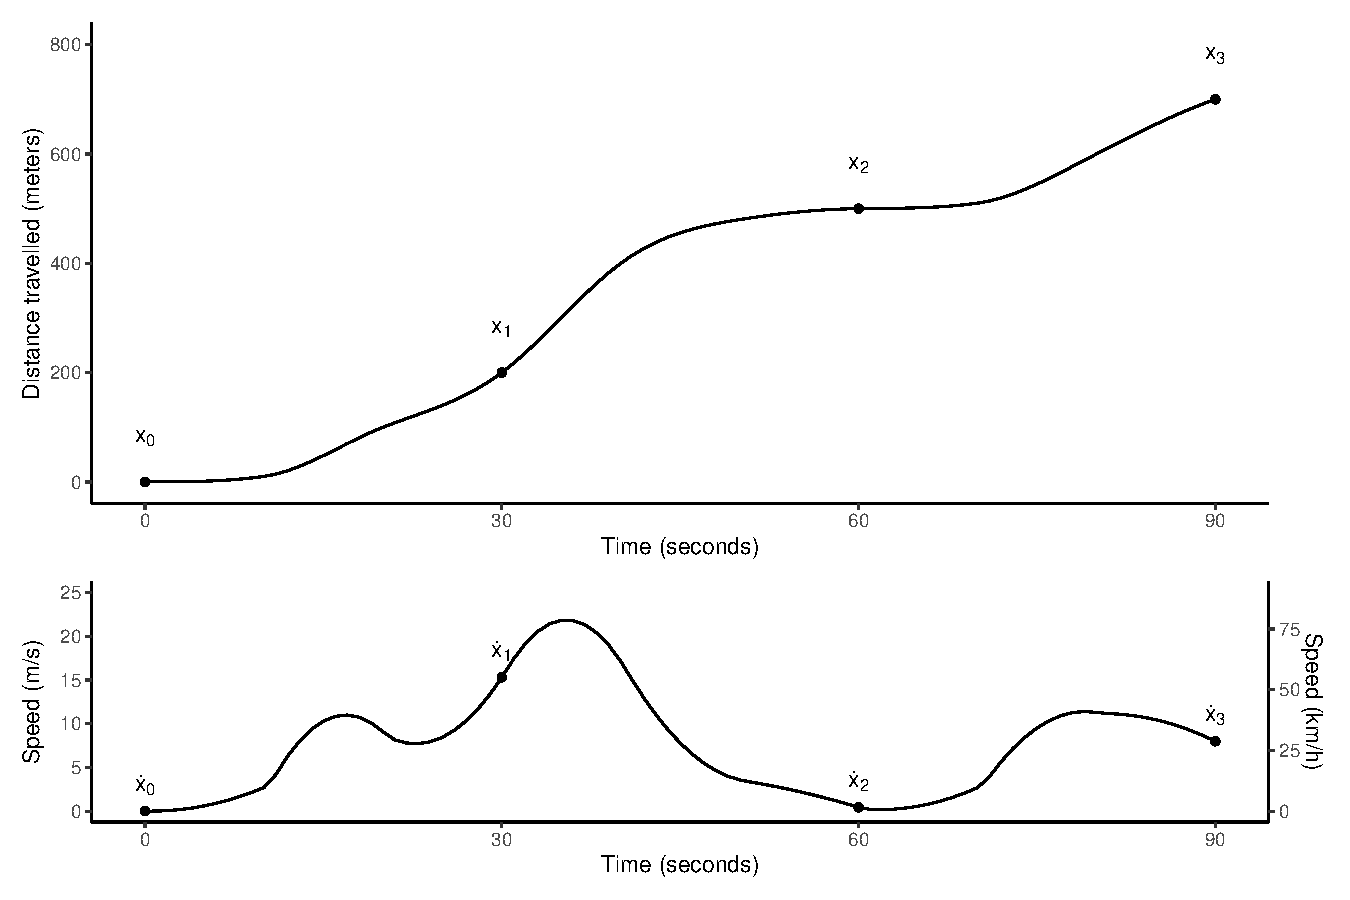
\includegraphics[width=\textwidth]{figure/vehicle_state-1} 

}

\caption[Visualisation of vehicle state showing \emph{distance travelled} and \emph{speed}]{Visualisation of vehicle state showing \emph{distance travelled} and \emph{speed}. The distance travelled, $x$, over time includes points of observed states $\Vstate_k, k=0,\ldots,3$. The gradient of distance over time is speed, $\dot x$: steeper sections of the top graph correspond to higher speeds, and vice verca. The speed graph also includes a second right-hand axis with speed in kilometers per hour (km/h) for reference.}\label{fig:vehicle_state}
\end{figure}


\end{knitrout}

The vehicle model itself involves describing bus behaviour algorithmically to infer the vehicle's \emph{unknown state} $\Vstate_k$ from a sequence of \gls{gps} observations. Since buses service routes with a known path, we represent their position using \emph{distance travelled} along the route's path, which we denote $\Vdist_k$ at time $\Vtime_k$. Additionally, we are interested in the \emph{speed} of the vehicle, $\Vspeed_k$. Therefore, the underlying, unknown, and \emph{unobservable} state of a vehicle at time t is denoted
\begin{equation}
\label{eq:vehicle_state}
\Vstate_k = \tvec{\Vdist_k, \Vspeed_k}.
\end{equation}
\Cref{fig:vehicle_state} graphs a series of vehicle states with time along the x-axis and distance travelled (in meters) along the y-axis. The derivative (gradient) of the curve represents the vehicle's speed. So, for example, the vehicle state at time $t_1 = 30$~seconds is $\Vstate_1 = [\Vdist_1, \Vspeed_1]^\top = [200~\text{m}, 15~\text{m/s}]^\top$. The remainder of this section presents a model, along with a particle filter implementation of it, which allows us to estimate vehicle state.

The particle filter represents the vehicle's state using a sample of \emph{particles}, each with an individual state, $\Vstate_k\vi$. We can think of each particle as an ``imaginary bus'' which represents one possible state (and associated trajectory) of the true bus. Together, the particles approximate the posterior distribution of the vehicle's state at time $\Vtime_k$ given all observations up to time $\Vtime_k$, denoted $\Vobs_{1:k}$. The posterior distribution is expressed using the Dirac delta measure, $\dirac_a$, (\cref{app:dirac-delta-measure}):
\begin{equation}
\label{eq:vehicle_state_dirac}
p(\Vstate_k | \Vobs_{1:k}) \approx
\sum_{i=1}^\Np \Pwt_{k-1} \dirac_{\Vstate_k\vi}\left(\Vstate_k\right).
\end{equation}

Before implementing \agls{rbm} for these data, we need a \emph{transition function}, a \emph{measurement function}, and a \emph{likelihood}. The transition function, $\Vtrans$, describes how a vehicle behaves between two consecutive observations: that is, the shape of the curve in \cref{fig:vehicle_state}. This allows us to \emph{predict} the future state of the vehicle \emph{given its last known state}. Additionally, we include the \emph{system noise} parameter $\Vnoise$, which represents the rate of change of speed. The measurement function, $\Vmeas$, describes the relationship between the vehicle's state, $\Vstate_k$, and the observation of this state, $\Vobs_k$, which is a \gls{gps} location with an associated \emph{measurement error}, $\GPSerr$. We represent this using two simple equations,
\begin{equation}
\label{eq:vehicle_model}
\begin{split}
\Vstate_k &= \Vtrans(\Vstate_{k-1}, \Vnoise_k) \\
\Vobs_k &= \Vmeas(\Vstate_k) + \GPSerr
\end{split}.
\end{equation}
The \emph{likelihood} function quantifies the plausibility of an observation $\Vobs_k$ given an underlying state $\Vstate_k$.


We now discuss the details of the two components of the model and their implementations. The \emph{prediction step} (\cref{sec:vehicle_model_trans}) supplies an estimate of the bus's state \emph{before observing it} by using a model of bus behaviour. Then the \emph{update state} (\cref{sec:pf-likelihood}) combines the prediction and observation, using the measurement function and likelihood, to obtain a posterior estimate of the vehicle's state.
